
%(BEGIN_QUESTION)
% Copyright 2010, Tony R. Kuphaldt, released under the Creative Commons Attribution License (v 1.0)
% This means you may do almost anything with this work of mine, so long as you give me proper credit

Determine the approximate value of the {\it derivative} ($dy \over dx$) for this function where $x=-8$:

$$\includegraphics[width=15.5cm]{i04380x01.eps}$$

Choose the closest answer:

\begin{itemize}
\item{} $dy \over dx$ = +1
\vskip 10pt 
\item{} $dy \over dx$ = $-1$
\vskip 10pt 
\item{} $dy \over dx$ = +2
\vskip 10pt 
\item{} $dy \over dx$ = $-2$
\vskip 10pt 
\item{} $dy \over dx$ = +5
\vskip 10pt 
\item{} $dy \over dx$ = $-5$
\vskip 10pt 
\item{} $dy \over dx$ = 0
\end{itemize}

\vskip 20pt \vbox{\hrule \hbox{\strut \vrule{} {\bf Suggestions for Socratic discussion} \vrule} \hrule}

\begin{itemize}
\item{} What is most important when solving problems such as this is to be able to explain {\it why} (not just {\it how}) to arrive at the correct value.  Try explaining the process of differentiation in your own words, as it applies to this particular problem.
\item{} Suppose the unit of measurement for $y$ is {\it dollars}, and the unit of measurement for $x$ is {\it hours}.  Identify the proper unit of measurement for $dy \over dx$, and a possible real-world application with these units that would fit the graph.
\end{itemize}

\underbar{file i04380}
%(END_QUESTION)





%(BEGIN_ANSWER)

$dy \over dx$ = 0

%(END_ANSWER)





%(BEGIN_NOTES)

\vfil \eject

\noindent
{\bf Prep Quiz:}

Determine the approximate value of the {\it derivative} ($dy \over dx$) for this function where $x=-3$:

$$\includegraphics[width=15.5cm]{i04380x01.eps}$$

Hint: the answer is an integer.








\vfil \eject

\noindent
{\bf Prep Quiz:}

Determine the approximate value of the {\it derivative} ($dy \over dx$) for this function where $x=5$:

$$\includegraphics[width=15.5cm]{i04380x01.eps}$$

Hint: the answer is an integer.








\vfil \eject

\noindent
{\bf Prep Quiz:}

Determine the approximate value of the {\it derivative} ($dy \over dx$) for this function where $x=10$:

$$\includegraphics[width=15.5cm]{i04380x01.eps}$$

Hint: the answer is an integer.










\vfil \eject

\noindent
{\bf Prep Quiz:}

Determine the approximate value of the {\it derivative} ($dy \over dx$) for this function where $x=0$:

$$\includegraphics[width=15.5cm]{i04380x01.eps}$$

Hint: the answer is an integer.


%INDEX% Mathematics, calculus: derivative (approximating derivative values at points on graph)

%(END_NOTES)


